\subsection{Beispiel 11}\label{ex:11}
Besonderheit: Das ist ein Grenzfall, der betont, dass die Reihenfolge der sortierten Rechtecke in den Listen $U_j$ eine wichtige Rolle spielt.
Dieser Fall zeigt auch, dass das vorgestellte Verfahren stark vereinfacht ist.
\vspace{.4cm}

Der Greedy--Algorithmus am Anfang liefert die Platzierung, die auf der \cref{fig:example11-1}
zu sehen ist. Das gelbe Rechteck wurde gewählt, da sein Wert $e_i$ am größten in der Liste 
$S_0$ ist. Als Nächstes wird die Lücke im Streifen 13, also direkt über dem gelben Rechteck,
im Verbesserungsverfahren gewählt, damit man in sie ein nicht gelegtes Rechteck platziert.
Das ist die einzelne Lücke in der Platzierung, die in einem Streifen liegt, in dem
mindestens ein Rechteck nocht nicht platziert ist.
In die gewählte Lücke wird das grüne Rechteck platziert.
So muss das gelbe kollidierende Rechteck entfernt sein. 
Es ensteht Platz für neue Rechtecke.
Nur aus dem Grund, dass das blaue Rechteck als erstes in der Liste $U_0$ steht, 
wird es platziert. So kommt es zur Platzierung aus der \cref{fig:example11-2}.
Da die Summe der Flächeninhalte der neuen Platzierung kleiner ist als die Summe 
der Flächeninhalte der alten Platzierung, wird die neue Platzierung vom Algorithmus abgelehnt.
Da dieser Algorithmus sehr stark vereinfacht ist, sucht man nicht nach Alernativen für
das blaue Rechteck. Die Lücke im Streifen 13 war die einzelne in der Platzierung und das grüne Rechteck
war das einzelne, das in diese Lücke eingefügt werden konnte. 
Aus diesem Grund bricht das Programm an dieser Stelle mit der Anfangsplatzierung als Endergebnis ab.
Die optimale Platzierung für dieses Beispiel ist auf der \cref{fig:example11-3} zu sehen.
\newpage

\noindent Der Flächeninhalt des großen Rechtecks: \framebox[1.1\width]{16 [m $\cdot$ h]}\\
Der Gesamtflächeninhalt aller platzierten Rechtecke: \framebox[1.1\width]{12 [m $\cdot$ h]}\\
Der Gesamtflächeninhalt aller Rechtecke: \framebox[1.1\width]{32 [m $\cdot$ h]}

\begin{figure}[hbt]
\centering
\begin{subfigure}[b]{0.32\textwidth}
\centering
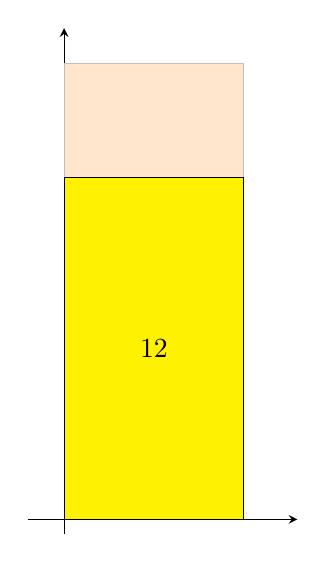
\begin{tikzpicture}
\begin{axis}[
		ticks=none,
        xmin =-.2,
        xmax = 1.3,
        ymax = 17.25,
        ymin = -0.5,
        width = 5cm,
        height = 8cm,
        axis x line = middle, axis y line = middle,
        every axis plot/.append style={ultra thick}]

	\draw [draw=lightgray, fill=orange, fill opacity=0.2] (0,0) rectangle node {$R$} (1, 16);
	\draw [fill = yellow] (0,0) rectangle node {12} (1,12);
	%\draw [fill = gray] (0,0) rectangle node {Streifen $S_0$} (10, 1) ;
	%\draw [fill = gray] (0,1) rectangle node {Streifen $S_1$} (10, 2) ;
	%\draw [fill = gray] (0,2) rectangle node {Streifen $S_2$} (10, 3) ;

	%\node[label={200:{$(0, 0)$}},circle,fill,inner sep=1.5pt] at (axis cs:0,0) {};
	%\node[label={200:{$(0, 12)$}},circle,fill,inner sep=1.5pt] at (axis cs:0,12) {};
	%\node[label={290:{$(N, B)$}},circle,fill,inner sep=1.5pt] at (axis cs:2,0) {};
	%\node[label={200:{$(0, E)$}},circle,fill,inner sep=1.5pt] at (axis cs:0,16) {};
	%\node[label={290:{$(N, E)$}},circle,fill,inner sep=1.5pt] at (axis cs:2,16) {};
	%\draw [fill = yellow] (0,7) rectangle node {} (5.26, 10) ;
\end{axis} 
\end{tikzpicture}

\caption{}
\label{fig:example11-1}
\end{subfigure}
%
\begin{subfigure}[b]{0.32\textwidth}
\centering
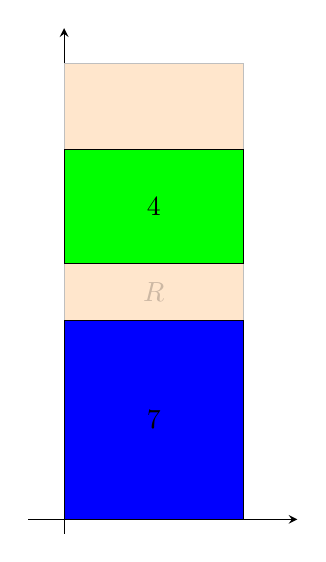
\begin{tikzpicture}
\begin{axis}[
		ticks=none,
        xmin =-.2,
        xmax = 1.3,
        ymax = 17.25,
        ymin = -0.5,
        width = 5cm,
        height = 8cm,
        axis x line = middle, axis y line = middle,
        every axis plot/.append style={ultra thick}]

	\draw [draw=lightgray, fill=orange, fill opacity=0.2] (0,0) rectangle node {$R$} (1, 16);
	\draw [fill = blue] (0,0) rectangle node {7} (1,7);
	\draw [fill = green] (0,9) rectangle node {4} (1,13);
	%\draw [fill = gray] (0,0) rectangle node {Streifen $S_0$} (10, 1) ;
	%\draw [fill = gray] (0,1) rectangle node {Streifen $S_1$} (10, 2) ;
	%\draw [fill = gray] (0,2) rectangle node {Streifen $S_2$} (10, 3) ;

	%\node[label={200:{$(0, 0)$}},circle,fill,inner sep=1.5pt] at (axis cs:0,0) {};
	%\node[label={200:{$(0, 7)$}},circle,fill,inner sep=1.5pt] at (axis cs:0,7) {};
	%\node[label={200:{$(0, 9)$}},circle,fill,inner sep=1.5pt] at (axis cs:0,9) {};
	%\node[label={200:{$(0, 13)$}},circle,fill,inner sep=1.5pt] at (axis cs:0,13) {};
	%\node[label={290:{$(N, B)$}},circle,fill,inner sep=1.5pt] at (axis cs:2,0) {};
	%\node[label={200:{$(0, E)$}},circle,fill,inner sep=1.5pt] at (axis cs:0,16) {};
	%\node[label={290:{$(N, E)$}},circle,fill,inner sep=1.5pt] at (axis cs:2,16) {};
	%\draw [fill = yellow] (0,7) rectangle node {} (5.26, 10) ;
\end{axis} 
\end{tikzpicture}
\caption{}
\label{fig:example11-2}
\end{subfigure}
%
\begin{subfigure}[b]{0.32\textwidth}
\centering
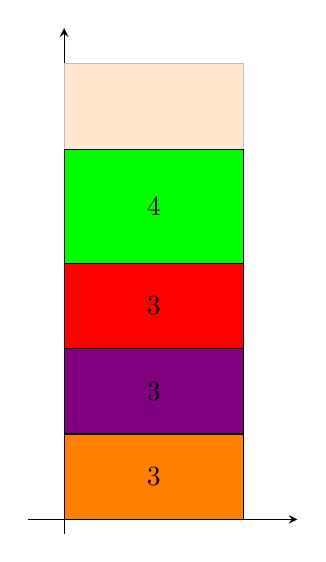
\begin{tikzpicture}
\begin{axis}[
		ticks=none,
        xmin =-.2,
        xmax = 1.3,
        ymax = 17.25,
        ymin = -0.5,
        width = 5cm,
        height = 8cm,
        axis x line = middle, axis y line = middle,
        every axis plot/.append style={ultra thick}]

	\draw [draw=lightgray, fill=orange, fill opacity=0.2] (0,0) rectangle node {$R$} (1, 16);
	\draw [fill = orange] (0,0) rectangle node {3} (1,3);
	\draw [fill = violet] (0,3) rectangle node {3} (1,6);
	\draw [fill = red] (0,6) rectangle node {3} (1,9);
	\draw [fill = green] (0,9) rectangle node {4} (1,13);
	%\draw [fill = gray] (0,0) rectangle node {Streifen $S_0$} (10, 1) ;
	%\draw [fill = gray] (0,1) rectangle node {Streifen $S_1$} (10, 2) ;
	%\draw [fill = gray] (0,2) rectangle node {Streifen $S_2$} (10, 3) ;

	%\node[label={200:{$(0, 0)$}},circle,fill,inner sep=1.5pt] at (axis cs:0,0) {};
	%\node[label={200:{$(0, 12)$}},circle,fill,inner sep=1.5pt] at (axis cs:0,12) {};
	%\node[label={290:{$(N, B)$}},circle,fill,inner sep=1.5pt] at (axis cs:2,0) {};
	%\node[label={200:{$(0, E)$}},circle,fill,inner sep=1.5pt] at (axis cs:0,16) {};
	%\node[label={290:{$(N, E)$}},circle,fill,inner sep=1.5pt] at (axis cs:2,16) {};
	%\draw [fill = yellow] (0,7) rectangle node {} (5.26, 10) ;
\end{axis} 
\end{tikzpicture}

\caption{}
\label{fig:example11-3}
\end{subfigure}
\caption{Die Zahlen in den Rechtecken 
stellen ihre Flächeninhalte dar.}
\label{fig:example11}
\end{figure}
